\chapter{Dark matter interpretations of Run 1 searches for invisibly decaying Higgs bosons}
\label{chap:interp}
As well as combining the results of the \ac{VBF} searches with other channels, it is also possible to interpret them as limits on other specific models. The particular models that are studied fall into two classes, \ac{EFT}s and simplified models, which are described in detail in \SectionRef{sec:DMextensions}. These studies were not carried out as part of the CMS collaboration, so it was necessary to develop and validate a framework for simulating the events resulting from these models.

%??CHECK PLOT AXIS LABEL SIZES AND THAT LEGEND TERMS ARE STANDARD OR IN TEXT

\section{Simulation Techniques and Validation}
\label{sec:dmval}
The CMS \textsc{Geant} based detector simulation is very computing intensive, so an alternative detector simulation with the \textsc{Delphes} fast reconstruction package was used. Whilst \textsc{Delphes} has been extensively validated by its authors against the CMS reconstruction~\cite{Favereau2014}, two of the variables used in the invisible Higgs boson decay searches described in this thesis are not implemented in the standard version of \textsc{Delphes}. Specifically, it was necessary to add a calculation of the \MET ignoring objects with $|\eta>3|$, to replicate the behaviour of the CMS \ac{L1} trigger, and it was also necessary to store the total transverse energy calculated using all particles in the event with no minimum threshold on their energy, which is required for the calculation of \METsig.

 Furthermore, whilst the signal process hard-scattering was simulated with Powheg in the CMS analysis, the studies described in this chapter use \textsc{MadGraph}. Both the internal CMS simulation and that described in this chapter use Pythia for parton-showering and hadronisation. Yields and kinematic distributions of events after selection criteria are applied are obtained from these simulations using an analysis framework developed and validated by the MasterCode collaboration~\cite{deVries:2015hva}.

%??start with internal sample validate against powheg plus delphes: when generated with same PU etc. found to agree to within 10% phenoplots281015.pdf
The validation of these simulations and the analysis framework was carried out in two steps. First, Powheg and pythia are used to simulate a \ac{VBF} produced 125 \GeV Higgs boson decaying to invisible final states, as in the internal CMS simulation. This sample of events is then processed using the \textsc{Delphes} based reconstruction and MasterCode analysis framework. The resulting event yields are compared to those obtained from a Powheg plus pythia sample processed using the full CMS reconstruction and analysis framework. The event yields were found to agree within 10\%.


The second step was to compare the 125 \GeV \ac{VBF} produces invisibly decaying Higgs boson sample generated with Powheg to one generated with \textsc{MadGraph} with both samples being processed using \textsc{Delphes}. This comparison was carried out starting from the following requirements:
\begin{equation}
  \label{eq:dmvalstart}
\eta_{j1}\cdot\eta_{j2}, \METsig>3, \detajj>3.6, \rm{leading\,and\,sub-leading\,jet\,}\pt>35 \GeV, \Mjj>700 \GeV, \rm{L1} \MET>40 \GeV.
\end{equation}
Cuts were then sequentially added to this selection until the applied selection was the same as the full Run 1 parked data \ac{VBF} Higgs to invisible search signal region selection, which is listed in \EquationRef{eq:parkedsigsel}. The resulting event yields can be seen in \TableRef{tab:mgvspowhegdelphes}. It is important to note that the \textsc{MadGraph} samples include both \ac{VBF} and \ac{VH} production of the Higgs boson, which explains the difference between the two samples being larger at the starting point of the comparison, and then reducing to below 5\% at the tighter steps of the selection where very few \ac{VH} events are still present. Only event yields after the full selection are used in the results presented in \SectionRef{sec:dmresults}, so the level of agreement is considered good.

%validate powheg plus delphes against mg plus delphes table from phenoplots281015.pdf
\begin{table}
  \caption{Event yields obtained, for several sets of event selection requirements, from two samples where the hard-scatter was simulated using \textsc{MadGraph} (second column) and Powheg (third column), both of which were processed using the \textsc{Delphes} fast detector reconstruction package. For each line the selection stated in the first column is added to the selection present for the line before. The starting point for the selection is described in \EquationRef{eq:dmvalstart}.}
  \label{tab:mgvspowhegdelphes}
  \begin{tabular}{lcc}
    \hline
    \hline
    Selection added & \textsc{MadGraph} + Delphes & Powheg + Delphes \\
    \hline
    Start point & 2653 & 2311 \\
    leading jet $p_{T}>50$ GeV, jet 2 $p_{T}>45$ GeV & 2056 & 1834 \\
    \METnoMU$>90$ GeV & 2000 & 1793 \\
    \Mjj$>1200$ GeV & 704 & 689 \\
    \METsig$>4$ & 539 & 519 \\
    \jetmetdphi$>2.3$ & 244 & 248 \\
    \hline
    \hline
  \end{tabular}
\end{table}

%??agreement can be seen to be good, the madgraph+delphes sim then used to generate samples at several mass points and for all the efts, met and eta for representative subsample of these shown in fig
Using the \textsc{MadGraph} hard-scattering plus \textsc{Delphes} detector reconstruction simulation, events from the signal models described in \SectionRef{sec:DMextensions} were generated. The distributions of \MET and leading jet $\eta$ for a representative sample of these models are shown in \FigureRef{fig:dmmodelkinematics}. It can be seen that whilst all of these models result in large values of \MET.

\begin{figure}
  \subfloat[]{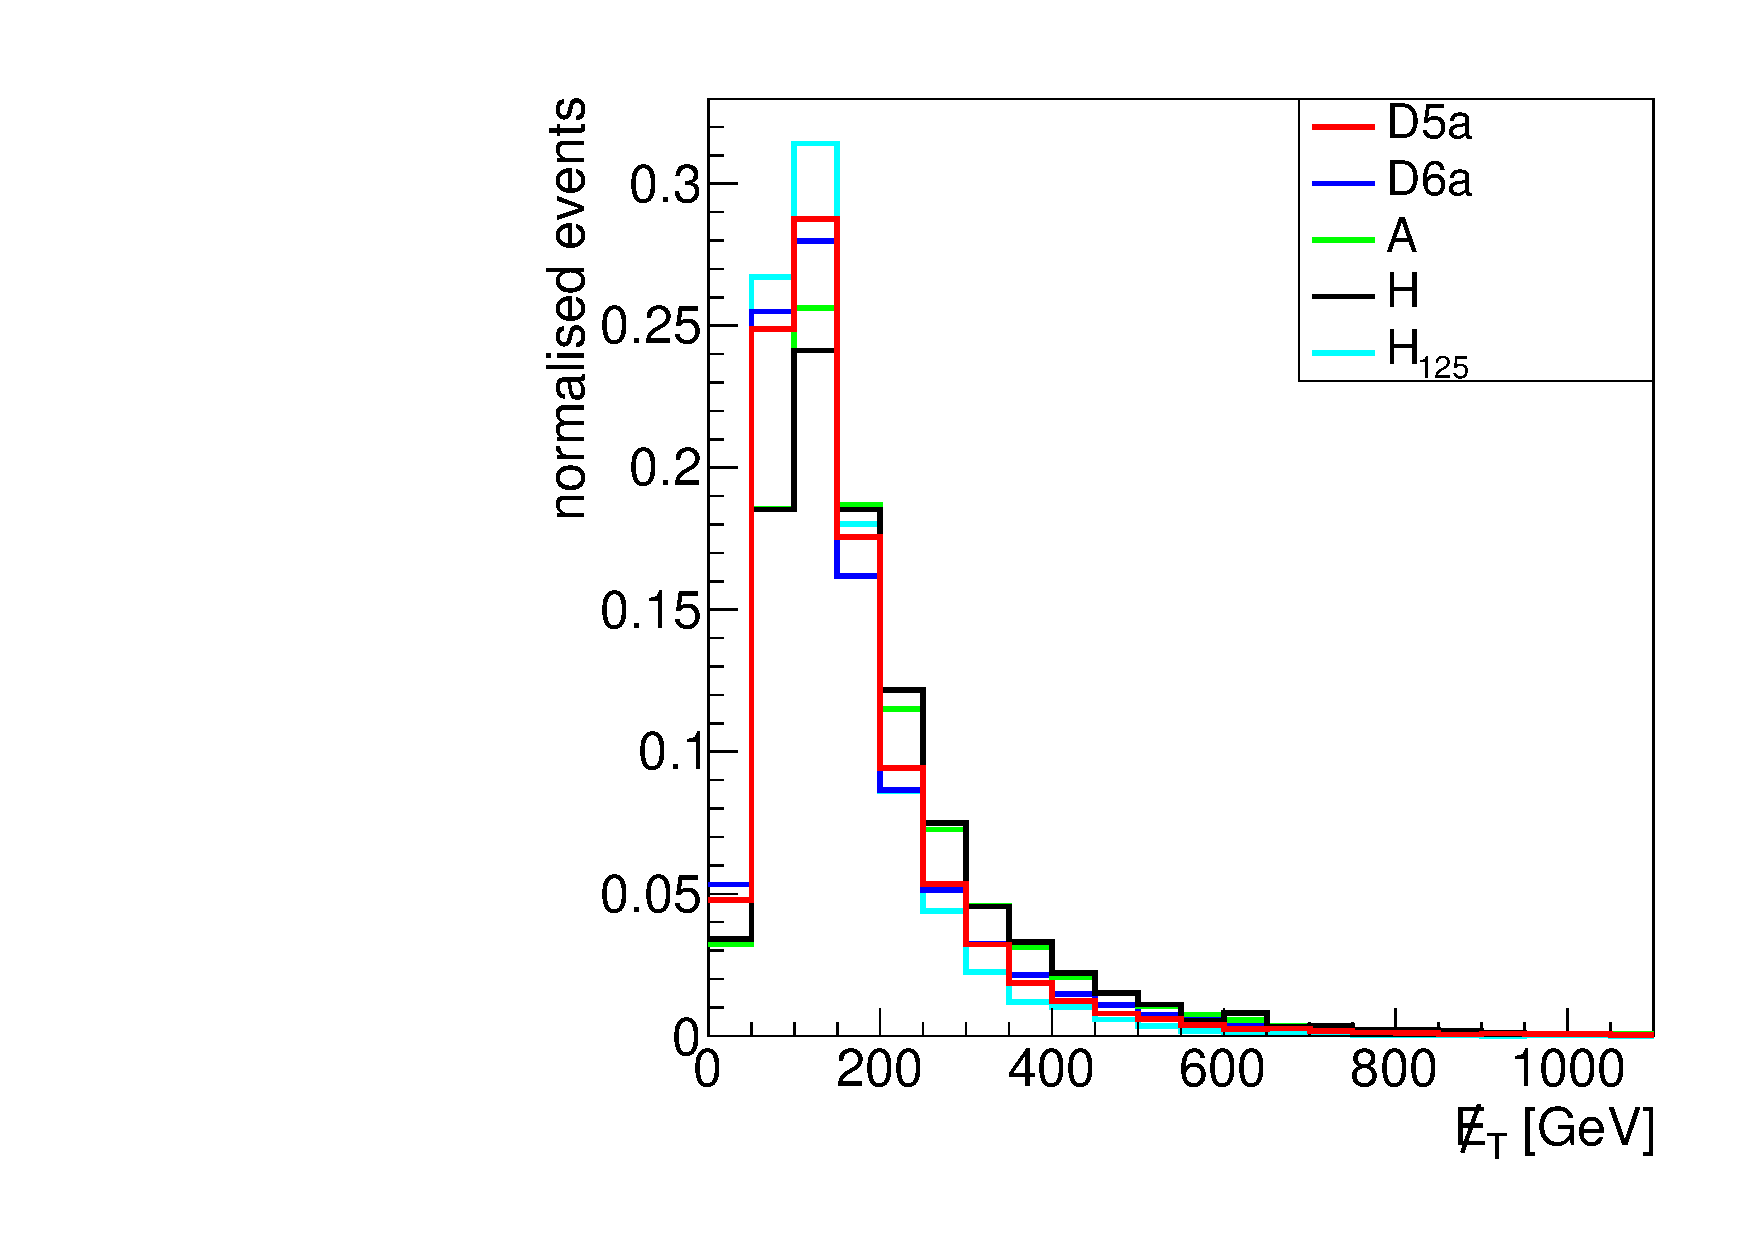
\includegraphics[width=.65\largefigwidth]{plots/interp/modelmet.pdf}}
  \subfloat[]{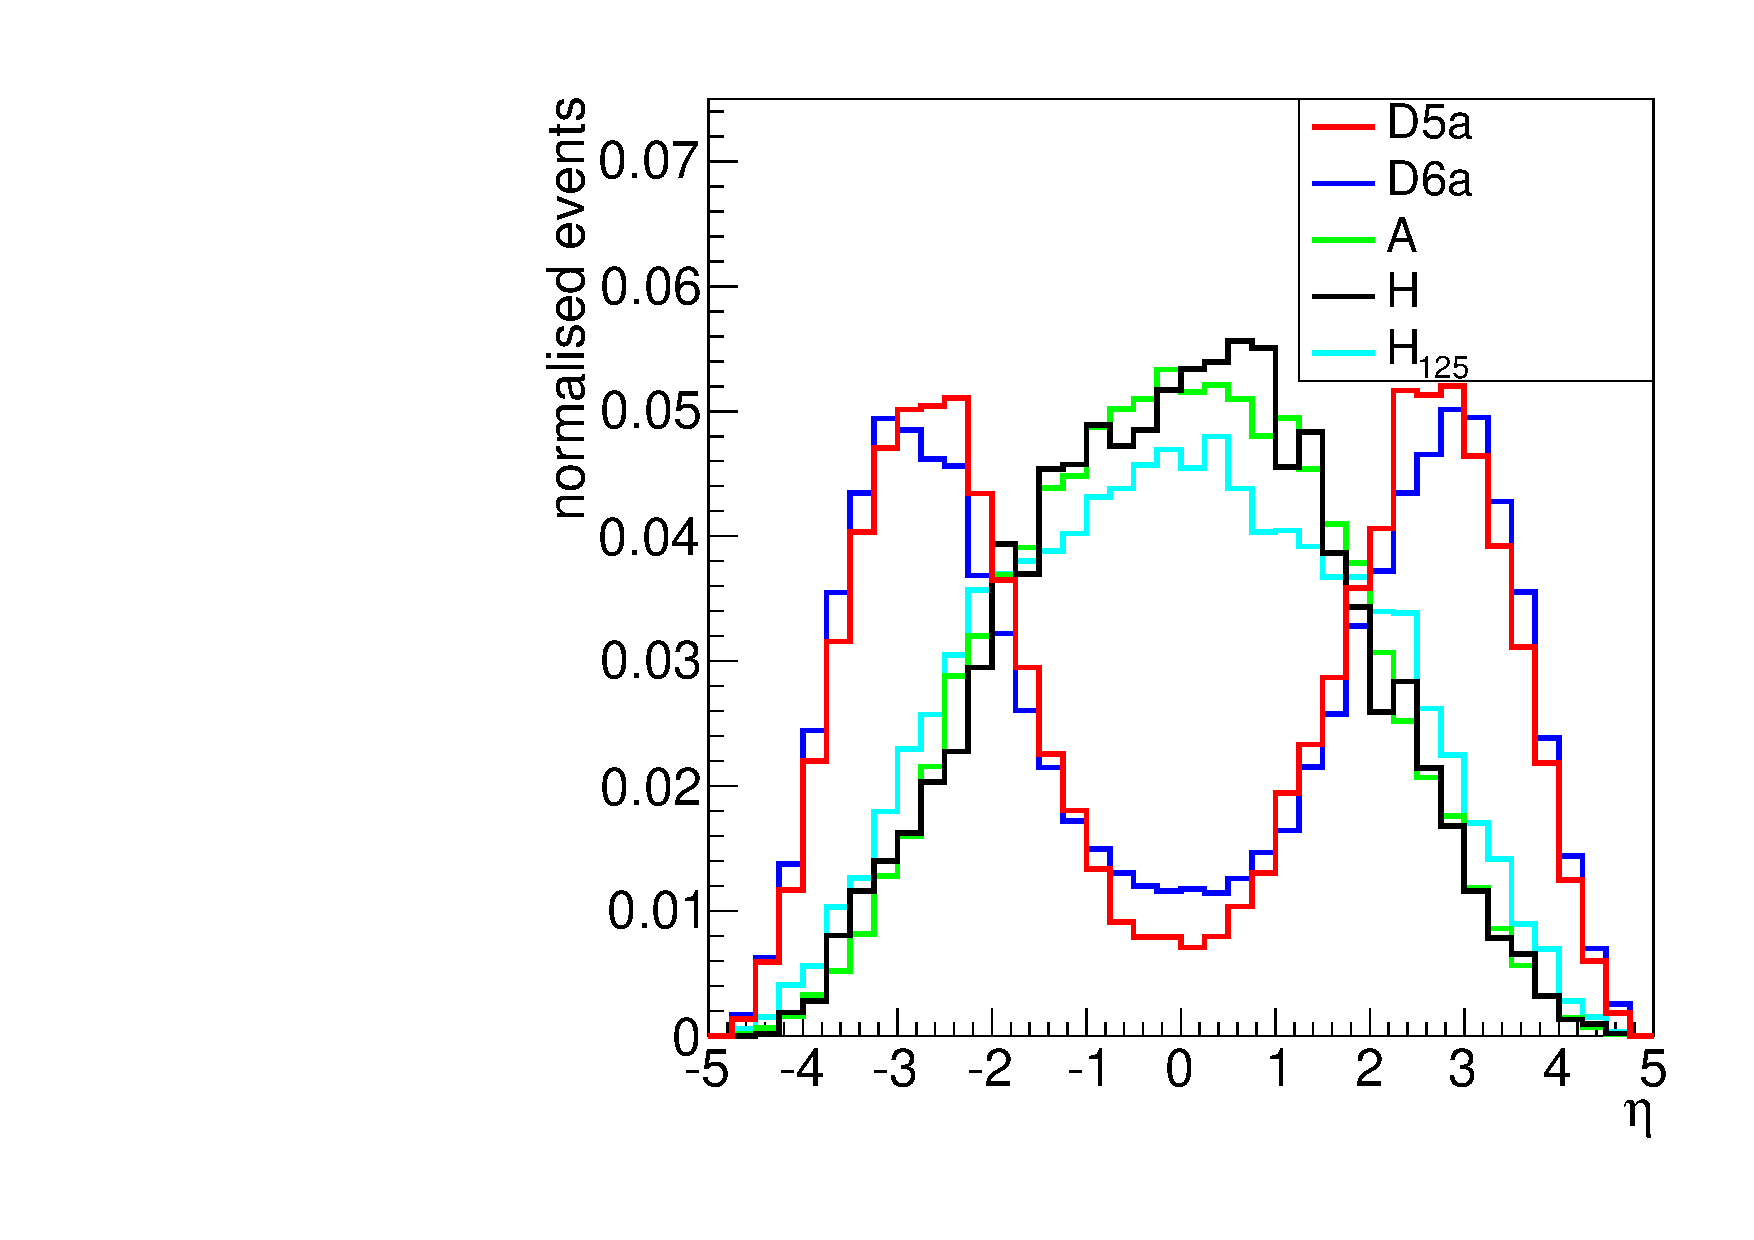
\includegraphics[width=.65\largefigwidth]{plots/interp/modeleta.pdf}}
  \caption{The \MET (a) and \eta of the leading jet (b), for two \ac{EFT} signal models (D5a and D6a), and spin-0 simplified models, described in \SectionRef{sec:DMextensions}, with representative model parameter values. For the \ac{EFT}s, heavier scalar (H) and pseudoscalar (A) models the dark matter mass, $m_{\chi}$ is assumed to be 100 \GeV, whereas for the 125 \GeV Higgs boson model $m_{\chi}$ is assumed to be 56.2 \GeV. For the scalar and pseudoscalar models the mass of the mediator is assumed to be 316.2 \GeV. It is important to note that the 125 \GeV Higgs boson model simulation includes \ac{VH} production of the Higgs boson as well as \ac{VBF}.}
  \label{fig:dmmodelkinematics}
\end{figure}

\section{Results}
\label{sec:dmresults}
%??first project 125 GeV higgs limits on and off-shell
%??systematic scaling, both shown for on-shell just lumi scale from then on

\begin{figure}
  \subfloat[]{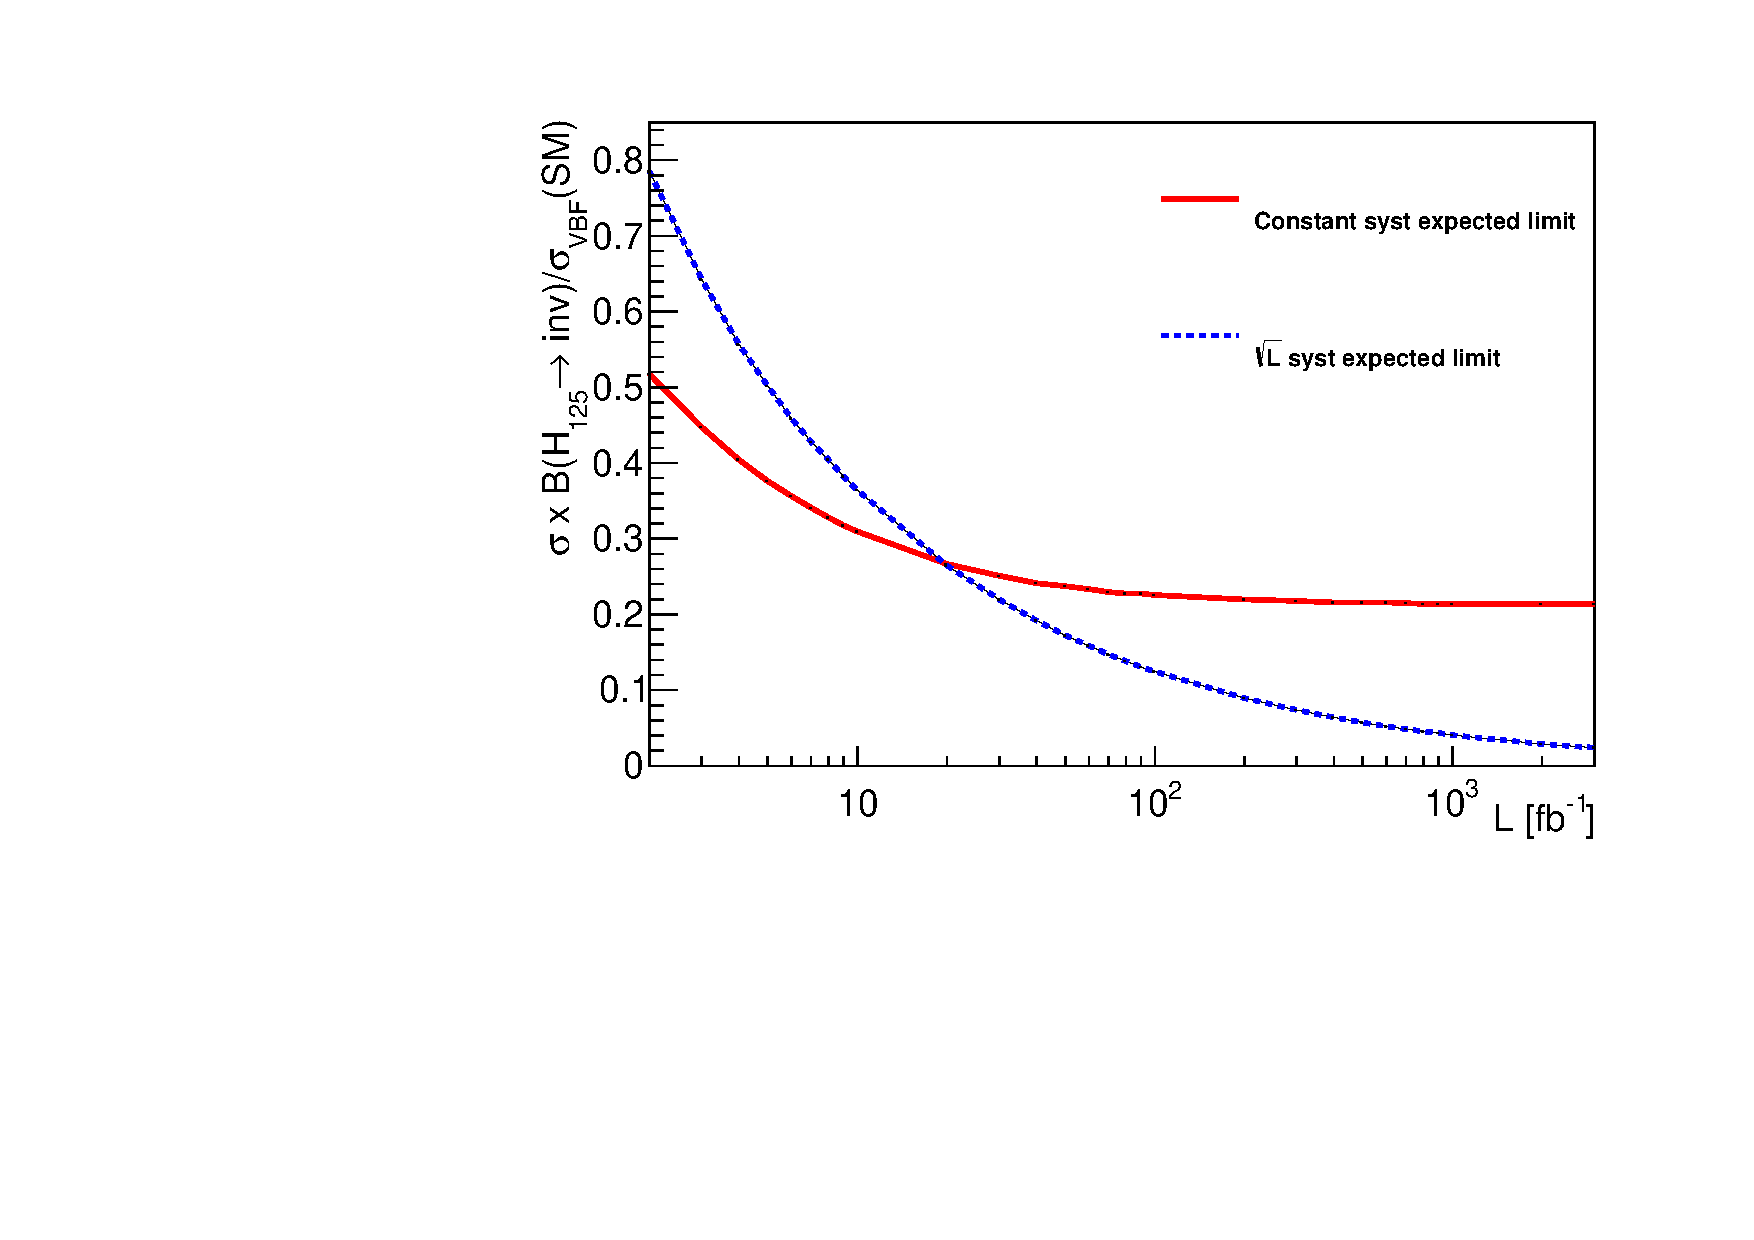
\includegraphics[width=\largefigwidth]{plots/interp/phenoprojectedvbflimit.pdf}}

  \subfloat[]{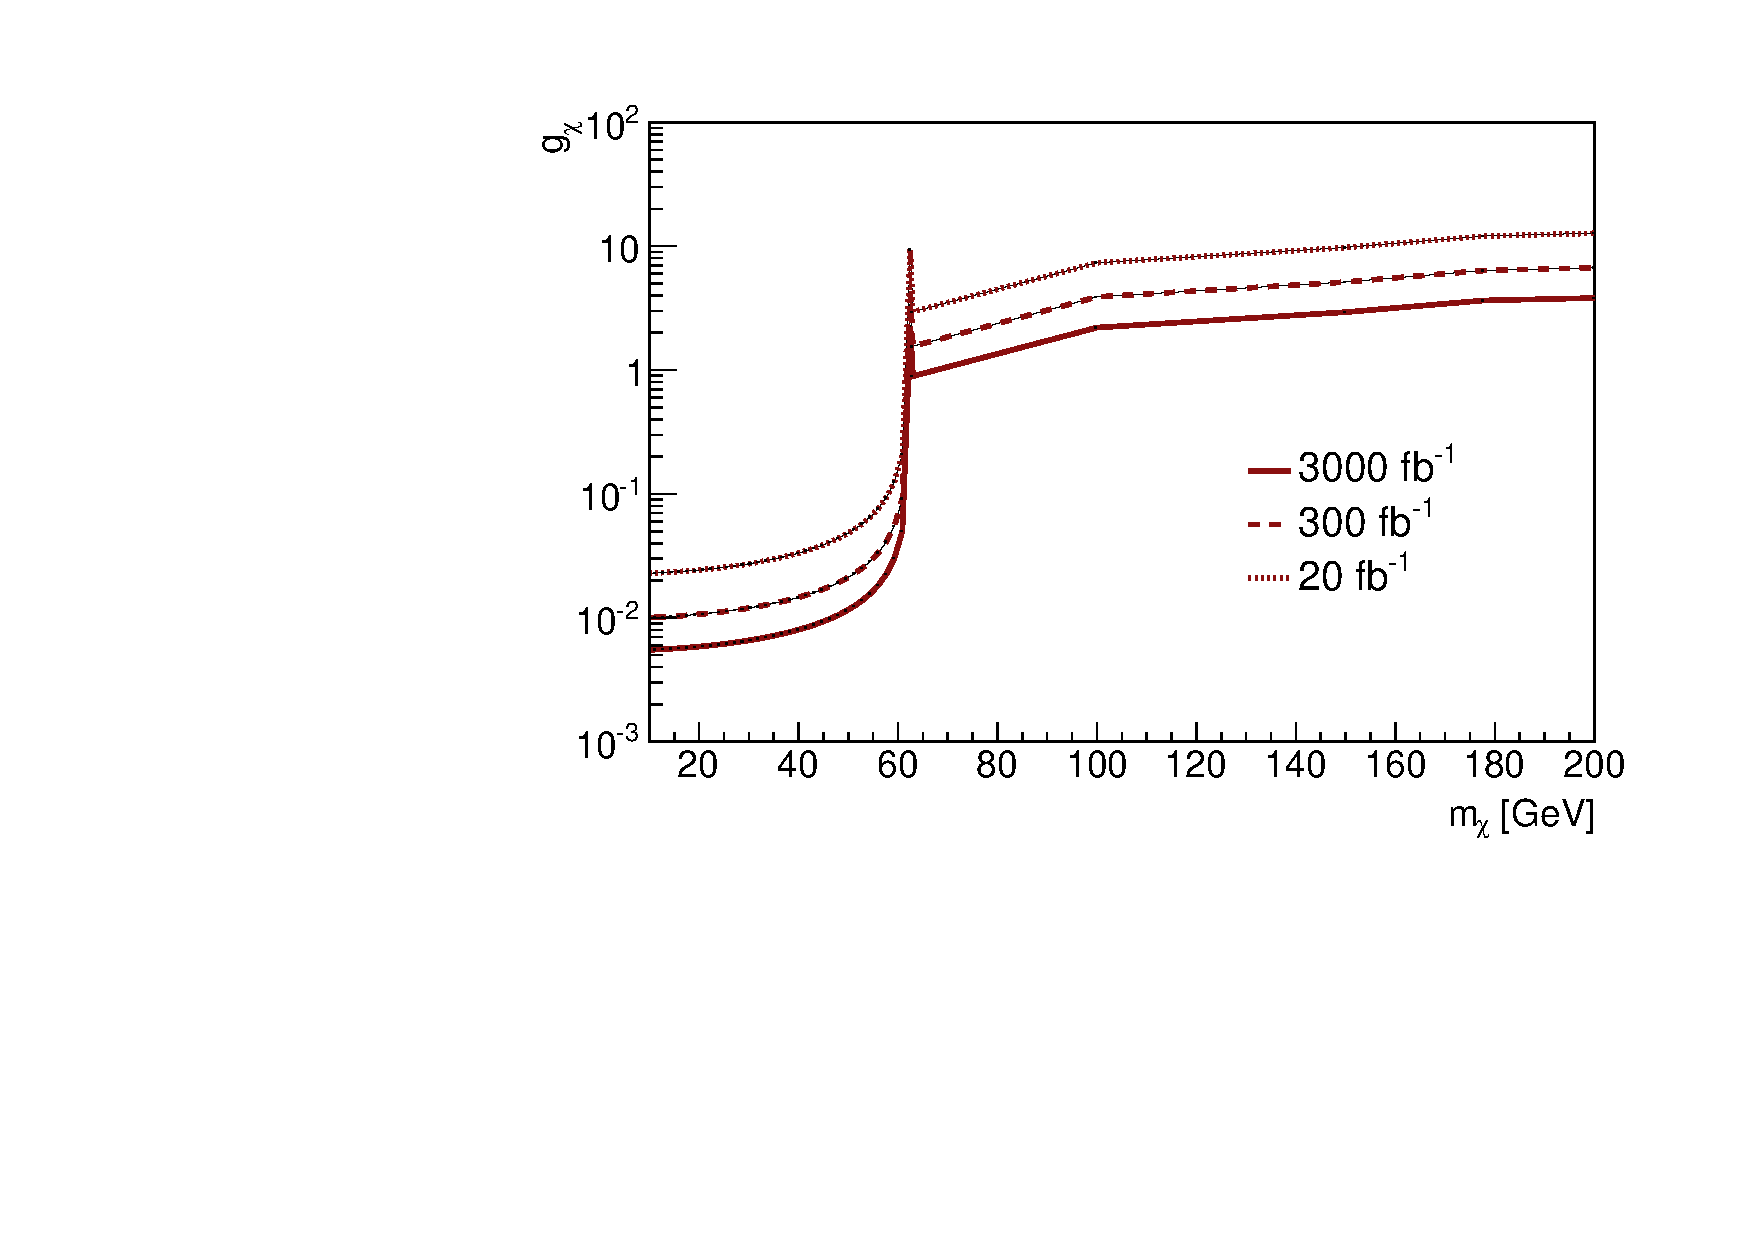
\includegraphics[width=\largefigwidth]{plots/interp/125higgsgchilimit.pdf}}
  \caption{}%??
  \label{fig:smprojectedlimits}
\end{figure}

%??non 125 GeV simplified models

\begin{figure}
  \subfloat[]{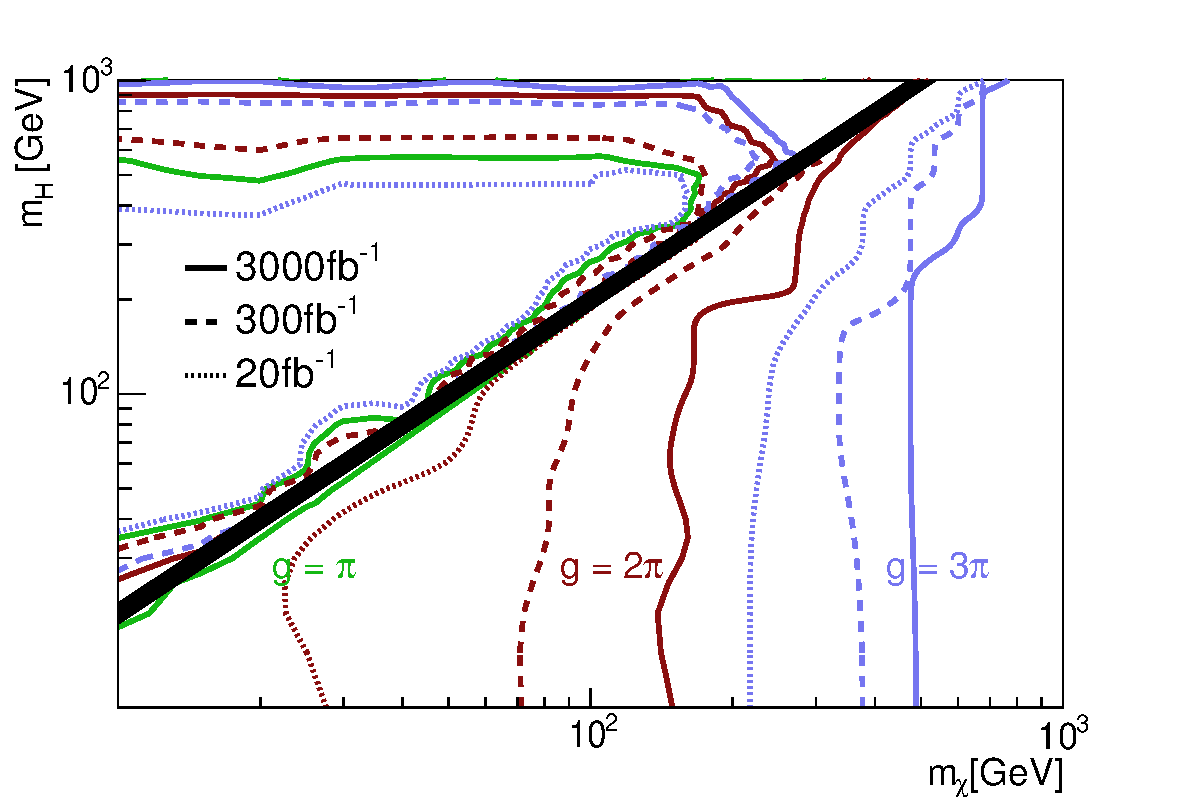
\includegraphics[width=\largefigwidth]{plots/interp/Hplane.pdf}}

  \subfloat[]{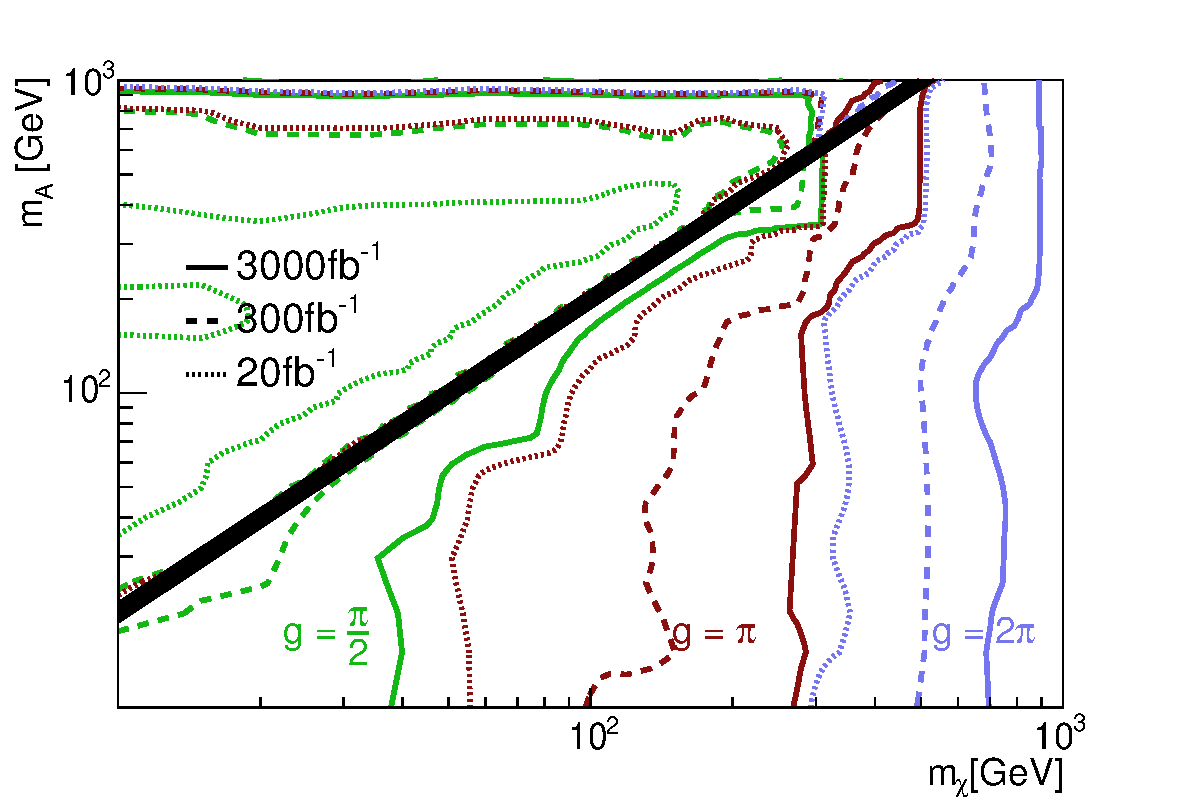
\includegraphics[width=\largefigwidth]{plots/interp/Aplane.pdf}}
  \caption{}%??
  \label{fig:simplifiedmodellimits}
\end{figure}

%??efts

\begin{figure}
  \subfloat[]{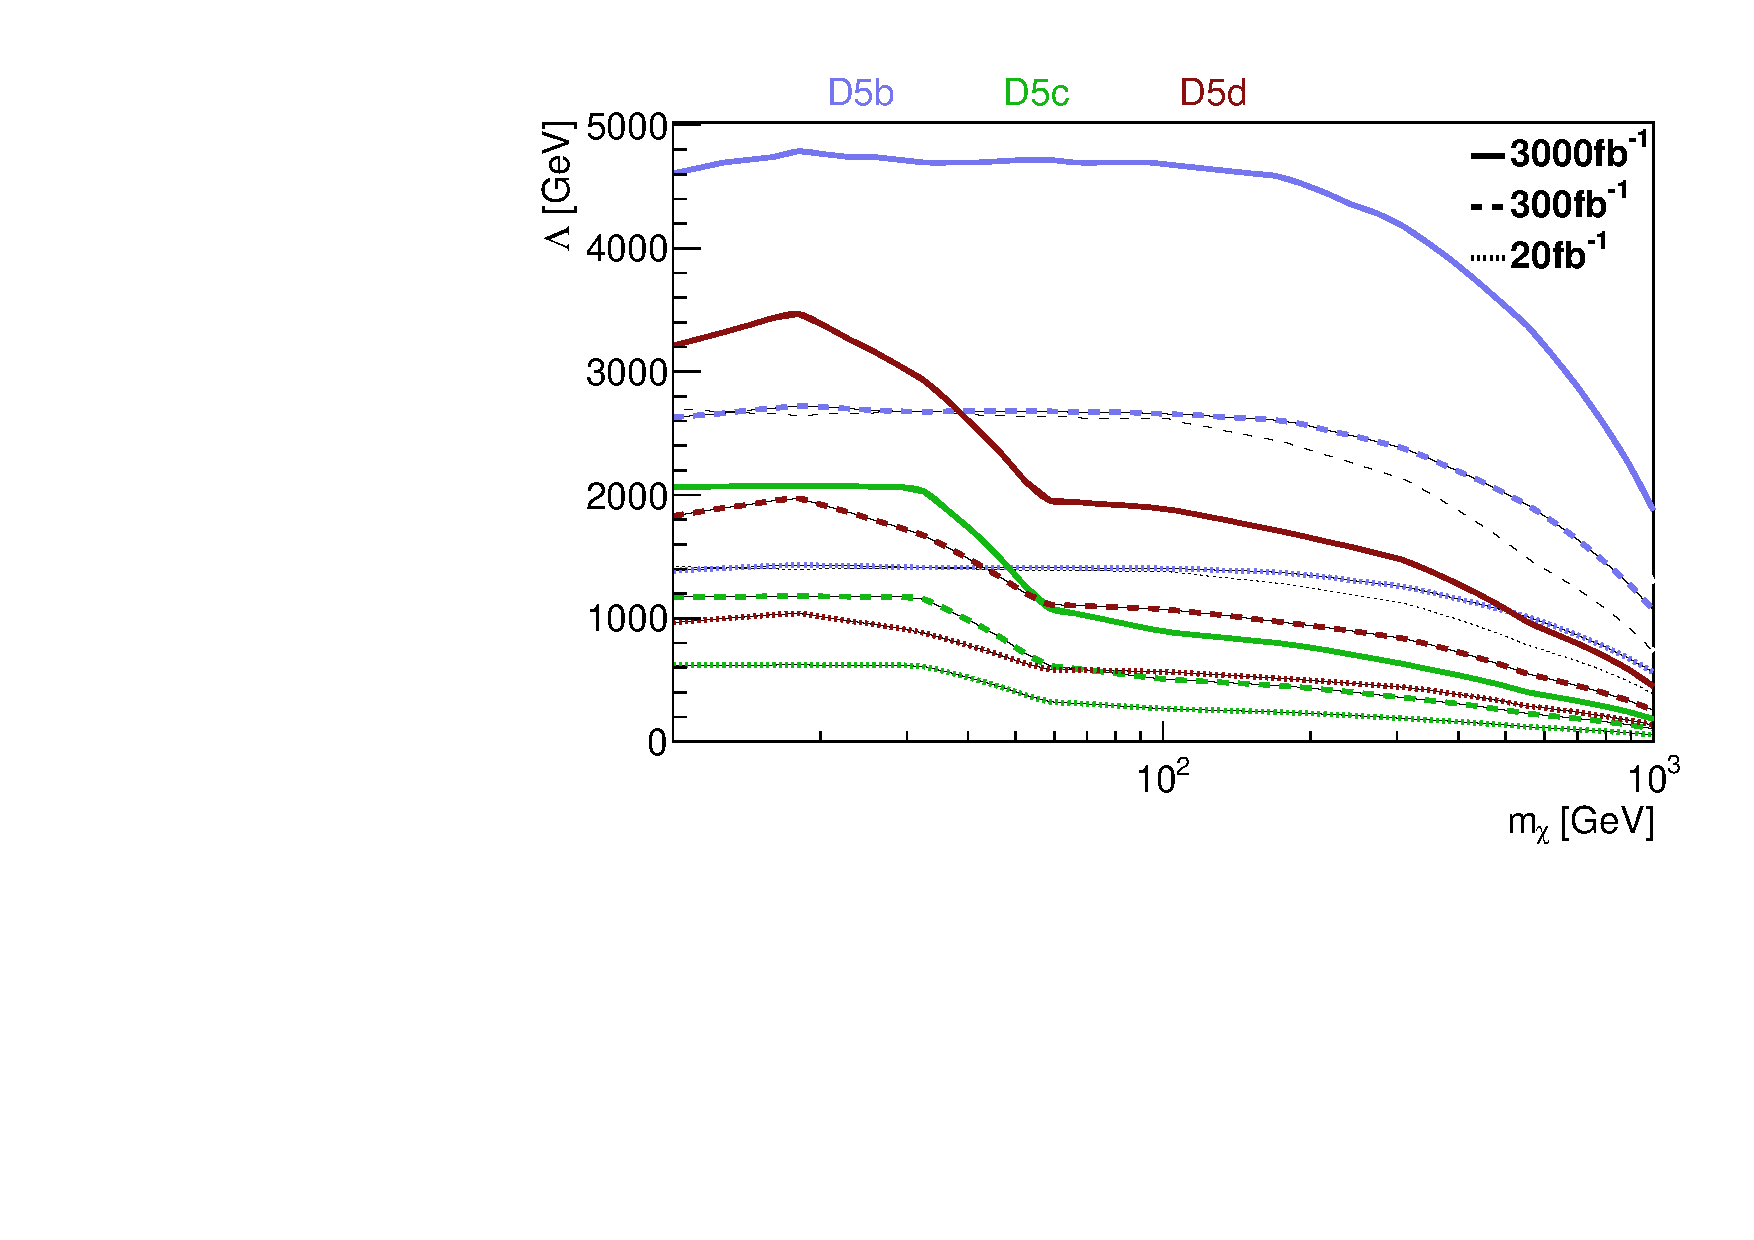
\includegraphics[width=.8\largefigwidth]{plots/interp/D5_multilumi.pdf}}

  \subfloat[]{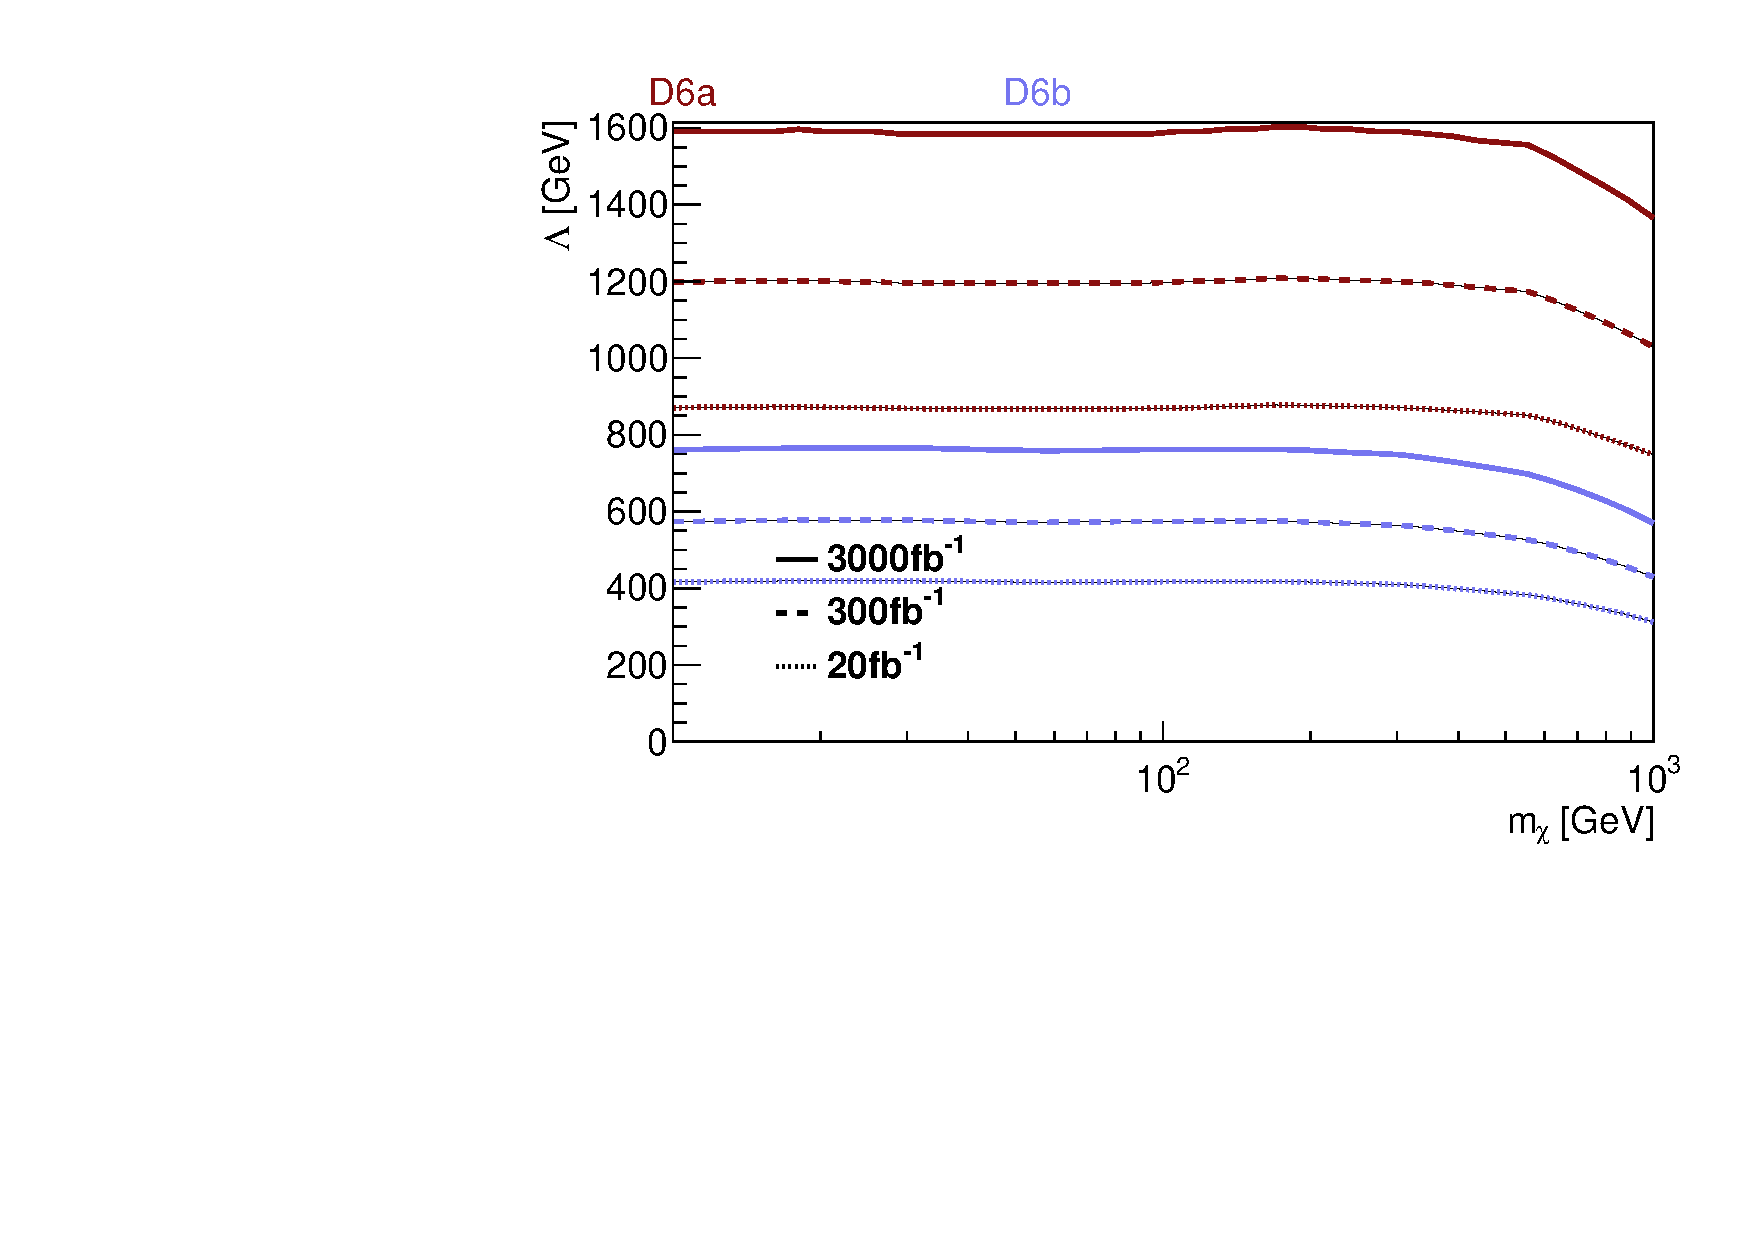
\includegraphics[width=.8\largefigwidth]{plots/interp/D6_2models.pdf}}

  \subfloat[]{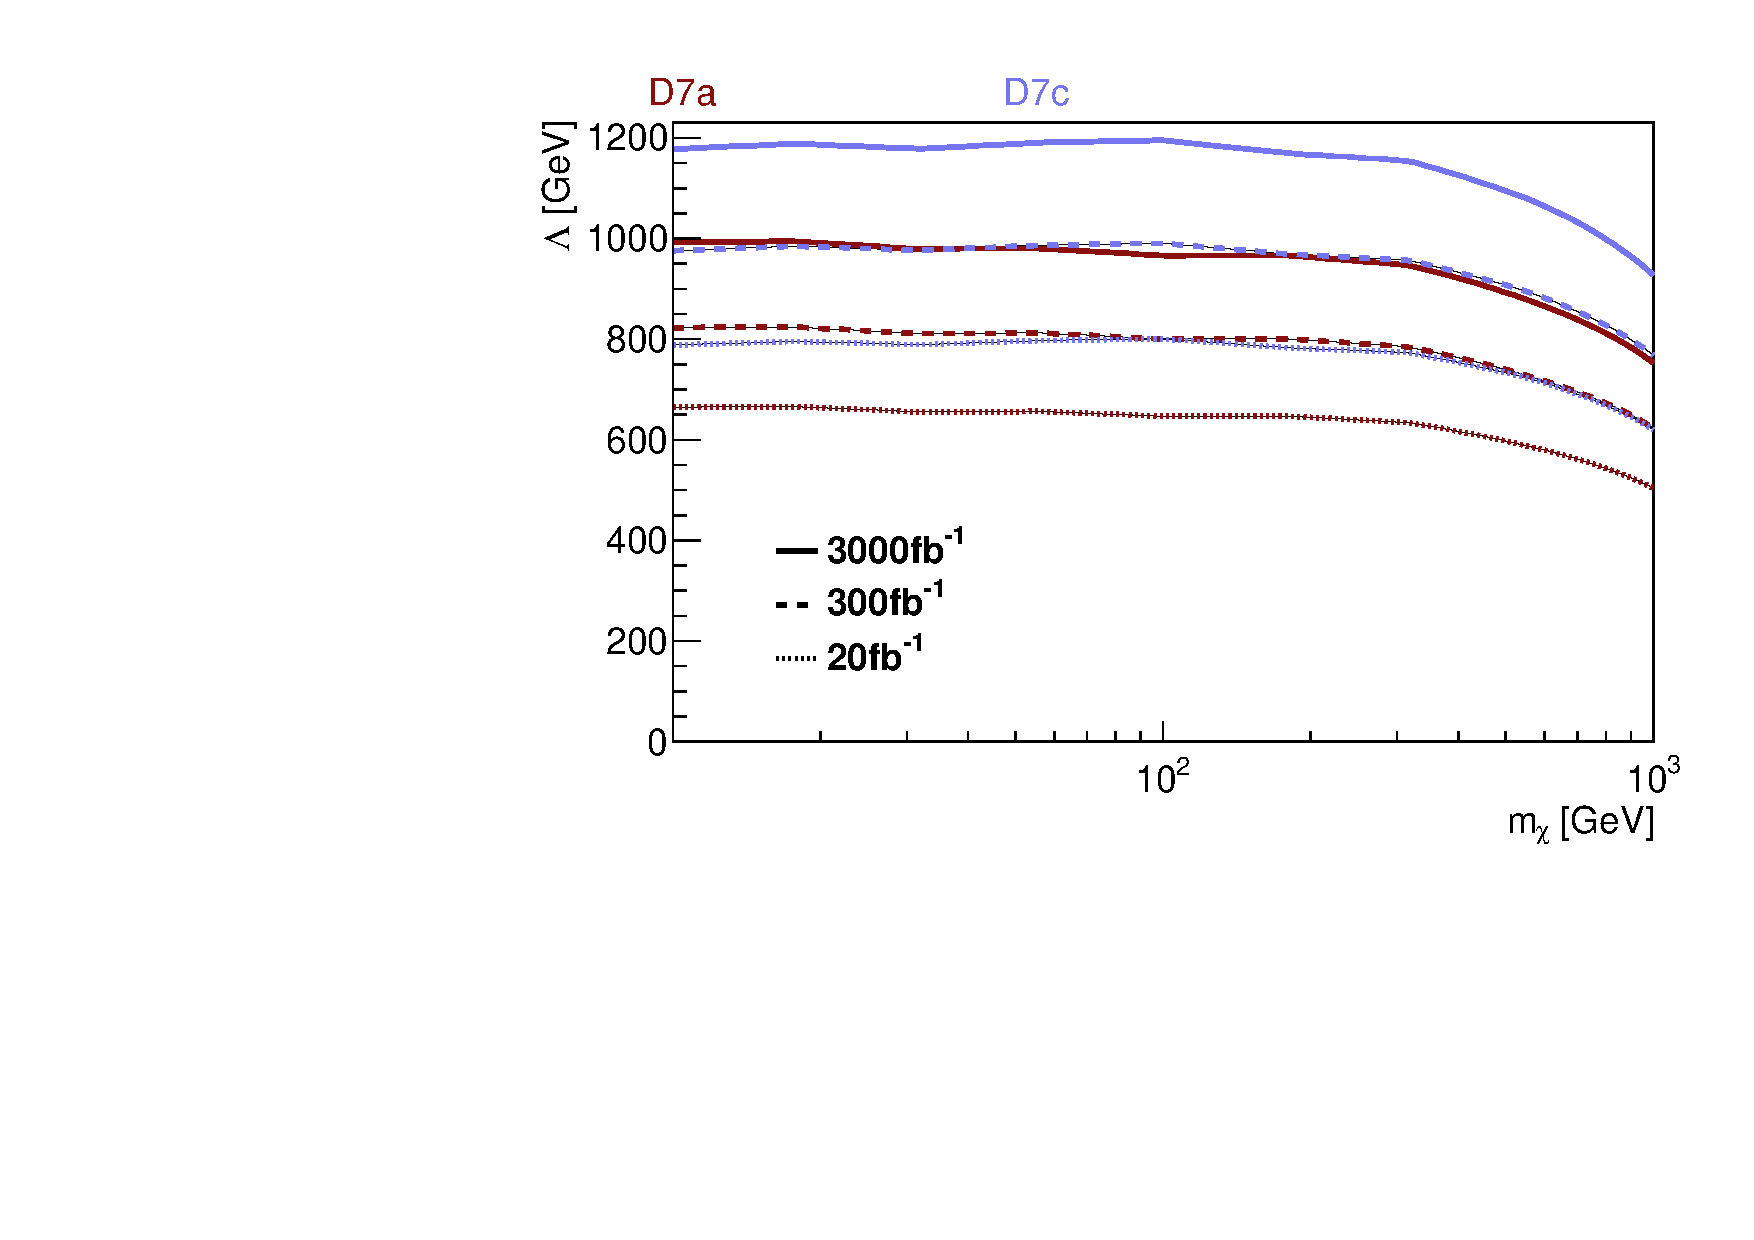
\includegraphics[width=.8\largefigwidth]{plots/interp/D7_2models.pdf}}
  \caption{}%??
  \label{fig:eftlimits}
\end{figure}

%??conclusion
